%\documentclass[letterpaper,12pt]{book}
%\usepackage[spanish]{babel}
%\usepackage{graphicx, color}
%\usepackage{amsmath}
%\usepackage{amscd}
%\usepackage{titlesec}
%\usepackage[latin1]{inputenc}
%\usepackage{listings}
%\usepackage{multicol}
%\usepackage{enumerate}
%\usepackage{amssymb}
%\usepackage{amsthm}
%\usepackage{syntonly}
%\usepackage{fancyhdr}
%\usepackage{verbatim}
%\usepackage{fancyvrb}
%\usepackage{hyperref}
%
%\begin{document}

%%%++++++++++++++++++++++++++++++++++++

Introducción histórica

\section{Fuerza magnética}
Una partícula de carga $q$, con velocidad $\vec{v}$ que entra a una región del espacio donde existe un campo magnético $\vec{B}$, siente una fuerza magnética:

\begin{equation}
\vec{F}_M=q \vec{v} \times \vec{B}
\end{equation}

\section{Fuentes de campo magnético}

Para completar la descripción de la interacción magnética, exploremos su origen.

\subsection{Ley de Biot-Savart}

Poco después de que Oersted descubriera la desviación de la aguja, Jean Baptiste biot y Felix Savart cuantificaron la fuerza magnética ejercida por un alambre sobre la aguja magnética. El hallasgo experimental, llamado la ley de Biot Savart, se resume en la siguiente expresión matemática.

\begin{displaymath}
\vec{B}=\dfrac{\mu_0 I}{4\pi}\int_l \dfrac{d\vec{l} \times \hat{u}_r}{r^2} ,
\end{displaymath}
donde $\mu_0=4\pi \times 10^{-7}$ T m/A, es una constante conocida como la permeabilidad del vacío.

\subsection{Ejemplos:}

\subsection*{Campo magnético de un alambre muy largo (infinito)}
Supongamos que tenemos un alambre delgado, muy largo y que transporta una corriente $I$ constante tal como se muestra en la Figura \ref{fig-alambreinfinito}.

\begin{figure}
\begin{center}
\includegraphics[scale=0.8]{magnetostatica/alambreinfinito}
\end{center}
\caption{Campo magnético de un alambre recto muy largo (infinito)}
\label{fig-alambreinfinito}
\end{figure}

\begin{eqnarray}
\nonumber
\vec{B}&=&\dfrac{\mu_0 I}{4\pi}\int_l \dfrac{d\vec{l} \times \hat{u}_r}{r^2} 
=\dfrac{\mu_0 I}{4\pi}\int_l \dfrac{dz\hat{k} \times \hat{u}_r}{r^2} \\ \nonumber
&=&\dfrac{\mu_0 I}{4\pi}\int_l \dfrac{dz\hat{k} \times (\sin\theta\hat{\rho} - \cos\theta \hat{k})}{r^2} 
=\dfrac{\mu_0 I}{4\pi}\int_{-\infty}^{\infty}\dfrac{dz\sin\theta }{r^2}\hat{u}_{\phi} \\ \nonumber
&=&\dfrac{\mu_0 I \rho }{4\pi}\int_{-\infty}^{\infty}\dfrac{dz }{(r^{2}+z^{2})^{3/2}}\hat{u}_{\phi} 
=\dfrac{\mu_0 I \rho }{4\pi}\Big[\dfrac{1}{\rho^{2}}\dfrac{z}{\sqrt{\rho^{2}+z^{2}}}\Big]\Big|_{-\infty}^{\infty} \hat{u}_{\phi} \\
&=&\dfrac{\mu_0 I}{2\pi\rho}\hat{u}_{\phi}
\end{eqnarray}

Note que el campo magnético rodea al alambre de acuerdo a la regla de la mano derecha. En general diremos que el campo magnético es un vector circulante en el sentido que está circulando alrededor del alambre. Además, note que el campo magético depende de la distancia radial al alambre, en este caso la variable $\rho$ (no se llamó $r$ para no generar confuciones a la hora de integrar).

\subsection*{Campo magnético de un alambre finito}

\begin{figure}[h]
\begin{center}
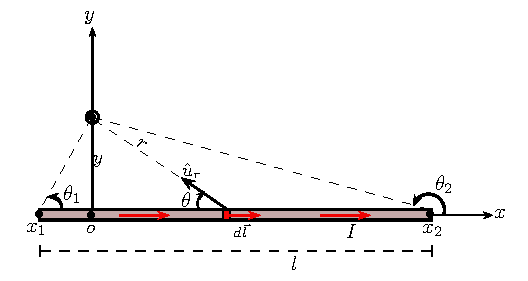
\includegraphics[scale=0.8]{magnetostatica/barra4}
\end{center}
\caption{Campo magnético de un alambre recto finito}
\label{fig-alambrefinito}
\end{figure}

De acuerdo a la Figura \ref{fig-alambrefinito}:

\begin{eqnarray}
\nonumber
\vec{B}&=&\dfrac{\mu_0 I}{4\pi}\int_l \dfrac{d\vec{l}\times \hat{u}_r}{r^{2}}
=\dfrac{\mu_0 I}{4\pi}\int_l \dfrac{dx \sin\theta}{r^{2}}\hat{k} 
=\dfrac{\mu_0 I y}{4\pi}\int_{-x_1}^{x_2} \dfrac{dx}{(x^{2}+y^{2})^{3/2}}\hat{k} \\ \nonumber
&=&\dfrac{\mu_0 I }{4\pi y}\Big(\dfrac{x_2}{\sqrt{x_2^{2}+y^{2}}} + \dfrac{x_1}{\sqrt{x_1^{2}+y^{2}}}\Big)\hat{k} \equiv  \dfrac{\mu_0 I }{4\pi y}(\cos\theta_1 -\cos\theta_2)\hat{k}
\end{eqnarray}

Note que si el alambre es infinito basta con tomar el límite cuando $x_1$ y $x_2$ tienden a infinito ó $\theta_1 =0^0$ y $\theta_2=\pi/2$. 

\subsection*{Campo magnético de un alambre circular}

\begin{figure}[h]
\begin{center}
\includegraphics[scale=0.8]{magnetostatica/campoB-anillo}
\end{center}
\caption{Campo magnético en el eje de un anillo de radio R}
\label{fig-campoB-anillo}
\end{figure}

De acuerdo a la Figura \ref{fig-campoB-anillo}, tenemos que:

\begin{eqnarray}
\nonumber
\vec{B}&=&\dfrac{\mu_0 I}{4\pi}\int_l \dfrac{d\vec{l}\times \hat{u}_r}{r^{2}}
=\dfrac{\mu_0 I}{4\pi}\int_l dl\dfrac{(\cos\theta \hat{k}+\sin\theta \hat{\rho})}{r^{2}} \\ \nonumber
&=&\dfrac{\mu_0 I}{4\pi}\Big[\int_l dl \dfrac{\cos\theta \hat{k}}{r^{2}}+\int_l dl \dfrac{\sin\theta \hat{\rho}}{r^{2}}\Big]
\end{eqnarray}
Dada la simetría del problema, el campo sólo sobrevive en la dirección $\hat{k}$ ($\int_l dl \hat{\rho}=\vec{0}$).

\begin{eqnarray}
\nonumber
\vec{B}&=&\dfrac{\mu_0 I}{4\pi}\int_l dl \dfrac{\cos\theta }{r^{2}}\hat{k}
=\dfrac{\mu_0 I}{4\pi} \dfrac{\cos\theta}{r^{2}} l \hat{k} 
=\dfrac{\mu_0 I}{4\pi} \dfrac{\cos\theta}{r^{2}} (2\pi R) \hat{k} \\
&=&\dfrac{\mu_0 I}{4\pi} \dfrac{R}{(R^{2}+z^{2})^{3/2}} (2\pi R) \hat{k}
=\dfrac{\mu_0 I}{2} \dfrac{R^{2}}{(R^{2}+z^{2})^{3/2}}\hat{k}
\end{eqnarray}

En general, el campo magnético de un alambre circular tiene una estructura muy complicada. En cualquier punto del espacio está descrito por la combinación de dos funciones muy especiales; los polinomios de Legendre y los armónicos esféricos. En la Figura \ref{fig-campomagneticoalambrecircular2} se muestran algunas de las líneas de campo. Note su similitud con las líneas de campo de imán de barra o del mismo planeta tierra.
 
\begin{figure}[h]
\begin{center}
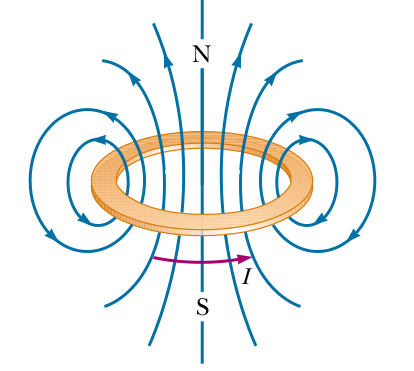
\includegraphics[scale=0.4]{magnetostatica/campomagneticoanillo}
\end{center}
\caption{Líneas de campo magnético de un segmento circular}
\label{fig-campomagneticoalambrecircular2}
\end{figure}

\subsection*{Campo magnético de un segmento circular de alambre}

Calculemos el campo $\vec{B}$ en el punto $O$ generado por el dispositivo mostrado en la Figura \ref{fig-segmentocircular}. Para ello, sólo es necesario calcular el campo magnético generado por el sector circular de ángulo $\theta$, ya que las secciones rectas no generan campo en el punto $O$.

\begin{figure}[h]
\begin{center}
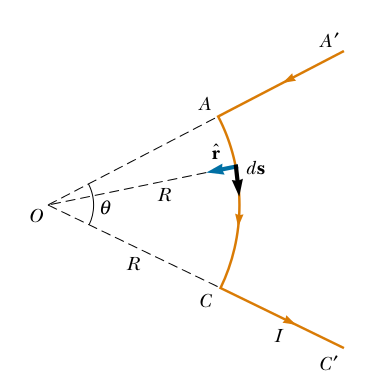
\includegraphics[scale=0.4]{magnetostatica/segmentocircular}
\end{center}
\caption{Campo magnético de un segmento circular}
\label{fig-segmentocircular}
\end{figure}

\begin{eqnarray}
\nonumber
\vec{B}&=&\dfrac{\mu_0 I}{4\pi}\int_l \dfrac{d\vec{s}\times \hat{u}_r}{r^{2}}
=\dfrac{\mu_0 I}{4\pi}\int_l \dfrac{ds}{r^{2}}
=\dfrac{\mu_0 I}{4\pi}\dfrac{1}{R^{2}} \int_l ds \otimes \\
&=&\dfrac{\mu_0 I}{4\pi}\dfrac{1}{R^{2}} (\theta R) \otimes
=\dfrac{\mu_0 I}{4\pi R}\theta \otimes ,
\end{eqnarray}

donde $\otimes$ indica que el campo está entrando de la hoja.

\subsection*{Campo magnético en el interior de un solenoide}

Consideremos un cilindró de radio $R$ y altura $l$ en el cual se enrrolla un alambre. Si suponemos que se tienen $N$ vueltas muy juntas, podemos pensar que en general se tiene una densidad de corriente que fluye circularmente alrededor del cilindro.\\
Usando el resultado obtenido para el campo magnético en el eje de una espira circular, tenemos que el diferencial de campo magnético $dB$ generado por un diferencial de corriente $dI$, es:

\begin{eqnarray}
dB=\dfrac{\mu_0 dI}{2}\dfrac{R^{2}}{(R^{2}+z^{2})^{3/2}}
\end{eqnarray}

Ahora, suponiendo que la densidad superficial de corriente es contante, entonces:
\begin{eqnarray}
\dfrac{dI}{dl}=\dfrac{dI}{dz}=\dfrac{NI}{l}=nI \Rightarrow dI=nIdz
\end{eqnarray}
Donde hemos definido la \textit{densidad de vueltas del solenoide} como:

\begin{equation}
n=(N/l)
\end{equation}

Usando lo anterior, tenemos que el campo magnético en el interior del solenoide es:

\begin{eqnarray}
\nonumber
B&=&\int_{-l/2}^{l/2}dB=\int_{-l/2}^{l/2}nI \dfrac{\mu_0}{2}\dfrac{R^{2}}{(R^{2}+z^{2})^{3/2}}dz \\ \nonumber
&=&\dfrac{\mu_0 nI}{2}	\int_{-l/2}^{l/2}\dfrac{R^{2}}{(R^{2}+z^{2})^{3/2}}dz
=\dfrac{\mu_0 nI}{2}\Big[\dfrac{z}{\sqrt{R^{2}+z^{2}}}\Big]\Big |_{-l/2}^{l/2}\\
&=&\dfrac{\mu_0 n Il}{\sqrt{l^{2}+4R^{2}}}
\end{eqnarray}

Generalmente los solenoides son largos, de tal modo que $l\gg R$. Así, en la expresión anterior:

\begin{eqnarray}
B \approx \mu_0 nI
\end{eqnarray}

Este resultado anterior será calculado de una forma más ráida cuando introduzcamos la Ley de Ampere.

\subsection*{Esfera rotante}

%%%++++++++++++++++++++++++++++++++++++
%\end{document}


